\documentclass{article}
\usepackage{color}
\usepackage{placeins}
\usepackage{listings}
\usepackage{graphicx}
\usepackage{xcolor}
\usepackage{amsmath}
\usepackage{subcaption}
\usepackage{cleveref}
\usepackage{geometry}[margins=1in]
\setlength{\parskip}{4pt plus 2pt}
\setlength{\parindent}{0pt}
%\pagecolor[rgb]{0,0,0} %black
%\color[rgb]{1,1,1} %grey
\lstset{language=C++,
keywordstyle=\color{blue},
stringstyle=\color{red},
commentstyle=\color{green},
morecomment=[l][\color{magenta}]{\#},
breaklines=true,
breakatwhitespace=true,
numbers=left
}
\title{Assignment \#5}
\author{Asbjørn Bonefeld Preuss,\\ Daniel Lomholt Christensen,\\ Elie Cueto}
\date{March 2024}

\renewcommand{\thesection}{Task \#\arabic{section}}
\renewcommand{\thesubsection}{\arabic{section}.\arabic{subsection}}
\begin{document}
\maketitle
\section{OpenACC parallelise the program}
The initial bottlenecks of the program without OpenACC was analysed using gprof. The result can be seen in figure \ref{fig:profiling:seq}. The profiling showed that efforts at parallelising the program should be focused around the integration function.
\begin{figure}[h]
    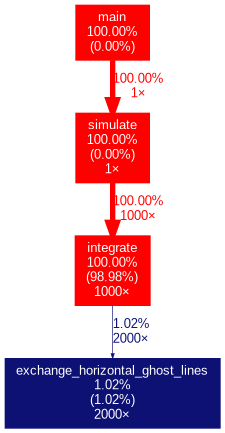
\includegraphics[width=0.5\textwidth]{./figures/sequential_profile.png}
    \centering
    \caption{Profiling of the sequential code, run with gprof and generated with gprof2dot.}
    \label{fig:profiling:seq}
\end{figure}
We initially had some loops running in parallel on the gpu. 
We did this by initialising a GPU accelerated region around the for loop of the simulation (line 155-164).
We here define which data is copied in, and must be copied out as well. In this function, the calculated version of water\_world.e is pushed to the cpu's version of water\_history.

On line 158 the integration function is called. In the integration function, the exchange horizontal and vertical ghost lines functions were quickly paralellised with acc parallel loop gang directives.

Next up, the integration function has two nested for loops, that are parallelized with parallel loop collapse.

With this setup we profiled the GPU accelerated code, and this result can be seen in figure \ref{fig:profiling:firstattempt}.
\begin{figure}[h]
    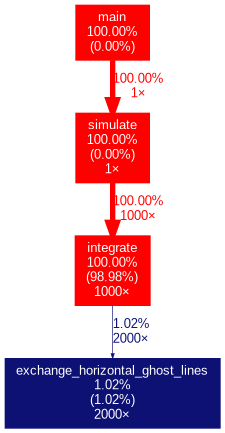
\includegraphics[width=0.5\textwidth]{./figures/sequential_profile.png}
    \centering
    \caption{Profiling of the first try to parallelise the code. }
    \label{fig:profiling:firstattempt}
\end{figure}

In the next attempt at optimization, we merged the two horizontal ghost line functions, as well as the two vertical ghost line functions, such that they calculate both w.e and w.u at the same time.

The initalisation of the accelerated region was also changed, such that it only copies in, not out. Finally, the integration loops gained an extra level of paralellisation by becoming parallel loop gang vectors instead of just parallel loops. This allows these used to be executed by gangs in vectors.

The results from this implementation can be seen in figure \ref{fig:profiling:secondattempt}
\begin{figure}[h]
    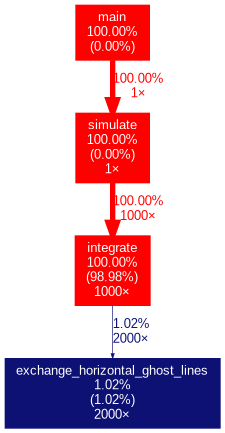
\includegraphics[width=0.5\textwidth]{./figures/sequential_profile.png}
    \centering
    \caption{Profiling of the second try to parallelise the code. }
    \label{fig:profiling:secondattempt}
\end{figure}

The third attempt focused on directing the compiler as to what data is already present on the GPU. This was done by the use of the present(variables) clause, which was put into the ghost functions, as well as the integration function.

Furthermore, the division of dt/dx and dt/dy in the integration function, was calculated a priori, such that we save those flops.

A profiling of this third attempt can be seen in figure \ref{fig:profiling:thirdattempt}
\begin{figure}[h]
    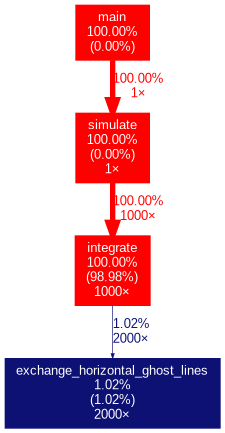
\includegraphics[width=0.5\textwidth]{./figures/sequential_profile.png}
    \centering
    \caption{Profiling of the third try to parallelise the code. }
    \label{fig:profiling:thirdattempt}
\end{figure}

The final attempt laid in only sending water\_history forth and back once between CPU and GPU, as well as parallelising a larger region at once, resulting in us optimising the synchronisation effort between individual GPU loops and the CPU, out of the program. 

\section{Strong and weak scaling using SLURM}



\FloatBarrier
\section{Source Code}
\label{sec:source}
\lstinputlisting[language=c++]{../Code/sw_parallel.cpp}

\end{document}
